\documentclass[10pt,twocolumn,a4paper]{article}
\usepackage[top=2cm,bottom=2.2cm,left=1.8cm,right=1.8cm,columnsep=0.6cm]{geometry}
\usepackage{fontspec}
\setmainfont{TeX Gyre Termes}
\usepackage{amsmath}
\usepackage{graphicx}
\usepackage{booktabs}
\usepackage{enumitem}
\usepackage[font=small,labelsep=colon,skip=4pt]{caption}
\usepackage{titlesec}
\titleformat{\section}{\large\bfseries}{\thesection}{0.6em}{}
\titleformat{\subsection}{\normalsize\bfseries}{\thesubsection}{0.6em}{}
\titlespacing*{\section}{0pt}{10pt}{4pt}
\titlespacing*{\subsection}{0pt}{8pt}{3pt}
\usepackage{url}
\usepackage{xurl}
\urlstyle{same}
\usepackage[hidelinks]{hyperref}
\setlength{\parindent}{1em}
\setcounter{dbltopnumber}{3}
\renewcommand{\dbltopfraction}{0.85}
\renewcommand{\topfraction}{0.85}
\renewcommand{\textfraction}{0.1}
\setlength{\textfloatsep}{10pt}
\setlength{\dbltextfloatsep}{10pt}
\renewcommand{\refname}{References}
\begin{document}
\twocolumn[
\begin{center}
{\LARGE\bfseries Why Federated Learning Falls Short\\[3pt] Across Hospitals\par}
\vspace{10pt}
{\large Đoàn Đức Nguyên (0009-0005-7460-8494)\par}
\vspace{2pt}
Department of Information Technology, FPT University\par
\vspace{12pt}
\begin{minipage}{0.86\textwidth}
\noindent\textbf{Abstract.} Federated learning lets hospitals train one skin-lesion classifier without sharing images. On real hospitals, however, it is often less accurate than training on all images in one place, and a trained model can still reveal which images were used to train it. We ask where the accuracy is lost and how much accuracy a formal privacy guarantee costs, treating the four image sources of HAM10000 as hospitals and using the six centres of Fed-ISIC2019 as a second test. When we rebuild the sites so that each holds images from all sources but keeps the same number of images per disease, models with batch normalization recover 35\% to 49\% of the accuracy they lose in federated training. Four further comparisons support our hypothesis that this loss enters through the batch-normalization statistics that the server averages across sites. A layer-normalization model is much less affected: ConvNeXt-atto reaches 0.741 balanced accuracy, against 0.661 for EfficientNet-B0, the model of the FLamby benchmark, and mixing the sources helps the benchmark model again on Fed-ISIC2019. For privacy, a strong membership attack still finds training images in federated models. With differential privacy, only training the last layer kept useful accuracy in our tests, and features learned from public dermoscopy images of another hospital raised accuracy at privacy level $\varepsilon = 3$ from 0.43 to 0.55, still 0.19 below the best model without this guarantee.
\end{minipage}
\vspace{16pt}
\end{center}
]

\section{Introduction}
A skin-cancer classifier needs many images of every lesion type, taken with many devices. A single clinic rarely has enough, and patient images usually cannot leave the hospital. Federated learning, or FL, lets hospitals train one model together [1]: each hospital trains the model on its own images, and a server averages the hospitals' models into one global model.

This has two known costs. Hospitals differ in their patients, diseases and imaging devices, and the averaged model is often less accurate than a model trained on all images in one place. Keeping images inside each hospital is also not a formal privacy guarantee, because a trained model can reveal whether a given image was used to train it. Differential privacy, or DP, gives such a guarantee, but it usually lowers accuracy further [2].

Studies of FL on skin images, such as the FLamby benchmark [3], mostly report how much accuracy is lost, averaged over hospitals. They do not test which difference between hospitals causes the loss, so it is unclear which fix to try. They also do not test with an attack whether keeping images on site actually protects patients.

We study both questions on HAM10000 [4], a dataset of skin images collected from four sources that we treat as four hospitals. To find out how much of the loss comes from differences between image sources, we rebuild the four sites so that each one mixes images from all sources while keeping the same number of images per disease, and we compare federated training on the real and on the mixed sites. We then compare models with different normalization layers to see where this loss enters the model, which leads to our best federated model. We repeat the main comparison on a second dataset, Fed-ISIC2019, and finally measure privacy and add DP. This work makes three contributions:
\begin{itemize}[leftmargin=*,itemsep=1pt,topsep=2pt]
\item It measures, on two datasets, how much of the accuracy lost in FL comes from differences between image sources, and gives evidence that this part enters through the batch-normalization statistics that the server averages.
\item It shows that a layer-normalization model loses less in FL and beats the benchmark model, and that this advantage appears only with enough training steps.
\item It shows that under DP, features learned from public images of another hospital raise accuracy, and it measures the accuracy that the guarantee still costs.
\end{itemize}

\section{Related work}
FL is known to lose accuracy when hospitals hold different data, and batch normalization has been reported to make this worse. Hsieh et al. [5] showed that averaging batch-normalization layers hurts when the label mix differs across sites, and FedBN [6] keeps these layers inside each site when the images of different sites look different. These studies mostly change the label mix or use different public datasets as sites; they do not test which real difference between hospitals causes the loss. For privacy, DP-SGD [2] limits and adds noise to the contribution of each image during training, Tramèr and Boneh [7] showed that under DP a linear classifier on good pretrained features can do better than training a whole network, and RMIA [8] is a recent membership attack that needs only a few extra models.

Table~\ref{tab:cmp} compares this work with the two studies closest to it, one for each of our datasets. FLamby is our baseline: it trains EfficientNet-B0 with FedAvg on Fed-ISIC2019. Our rerun of this setup gives 0.624, against 0.539 with a standard deviation of 0.097 over five seeds in the results that FLamby released, so our run lies within their range. FLamby trains for a fixed, short number of steps, and Section~\ref{sec:best} shows that with this number of steps the layer-normalization model shows no advantage. Chen et al. [9] also use real dermoscopy sources as sites, but with three classes and a different metric, so their numbers cannot be compared with ours directly. Neither study measures which part of the accuracy loss comes from differences between image sources, or tests privacy with an attack.

\begin{table*}[t]
\caption{This work and the two closest studies.}\label{tab:cmp}
\centering\small
\begin{tabular}{lllll}
\toprule
Study & Data & Sites & Accuracy reported & Privacy attack \\
\midrule
FLamby [3] & Fed-ISIC2019, 8 classes & 6 centres & mean over centres & no \\
Chen et al. [9] & HAM10000 and MSK, 3 classes & 4 sources & macro F1 and AUC & no \\
This work & HAM10000 and Fed-ISIC2019 & 4 sources, 6 centres & share lost to source differences & membership attack \\
\bottomrule
\end{tabular}
\end{table*}

\section{Method}
Figure~\ref{fig:pipe} shows the pipeline that every experiment follows; experiments differ only in what is used in each box. The training images are first split into $K$ sites. At each site, images are preprocessed, augmented and passed through a backbone, which is a stack of blocks each followed by a normalization layer, and then through a linear classifier. In the local update, each site trains this network on its own images for one epoch. Each site then sends its model to the server, which averages the $K$ models, giving more weight to larger sites, and sends the result back as the starting point of the next round. The final model is scored for accuracy and attacked to test privacy. Centralized training, our reference, trains the same network on all images in one place, without sites or a server. The study varies three boxes: the site split, the normalization layer and, for privacy, the local update, whose private version is shown in Figure~\ref{fig:design}.

\begin{figure*}[t]
\centering
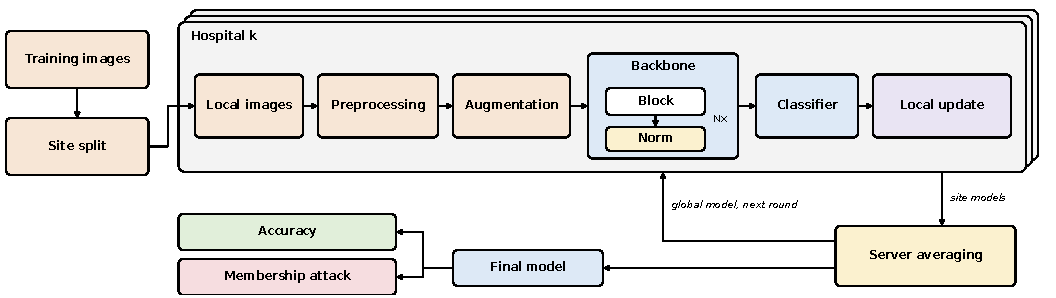
\includegraphics[width=\textwidth]{figures/fig1_pipeline.pdf}
\caption{Pipeline shared by all experiments. The study varies the site split, the normalization layer and the local update.}\label{fig:pipe}
\end{figure*}

\begin{figure*}[t]
\centering
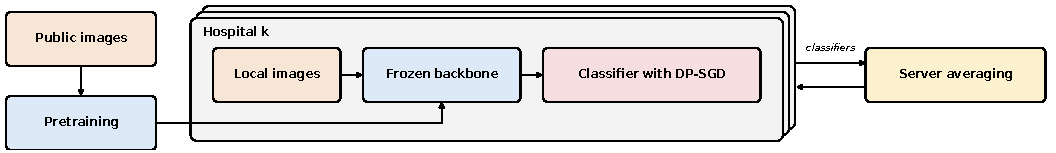
\includegraphics[width=\textwidth]{figures/fig3_design.pdf}
\caption{Proposed private version of the local update. A backbone trained on public dermoscopy images is frozen; each site trains only the classifier with DP-SGD, and the server averages the classifiers.}\label{fig:design}
\end{figure*}

\subsection{Real and mixed sites}
HAM10000 has 10,015 dermoscopy images of 7,470 lesions in seven disease classes, collected from four sources: three collections of the Department of Dermatology in Vienna, which we call molemax, modern and dias, and one practice in Queensland, Rosendahl. We treat each source as a site because each is a real clinic or imaging setup. The sites differ nine-fold in size, from 365 to 3,388 training images, and in their diseases: 94\% of the molemax images are benign nevi, and two sites have no image of actinic keratosis. We split training and validation images by lesion, so that photos of the same lesion never appear in both, which gives 8,583 training and 1,432 validation images. Each final model is also scored once on the official ISIC 2018 test set of 1,512 images. Because 67\% of the images are nevi, we report balanced accuracy: the recall of each class averaged over the seven classes, so that a model cannot score well by always predicting the largest class.

Images from different sources look different even for the same disease. Figure~\ref{fig:nevi} shows benign nevi from each site: colour, skin tone and the borders of the dermoscope change with the source. Using only six colour statistics of benign nevi, a logistic regression predicts which source an image came from with accuracy 0.80, where guessing gives 0.25. The sources may differ in their patients and photography habits as well as in their devices. We expect the devices to matter most, because the two large Vienna sources come from the same department but used different devices, and a logistic regression on strips of healthy skin tells them apart with accuracy 0.99.

\begin{figure}[t]
\centering
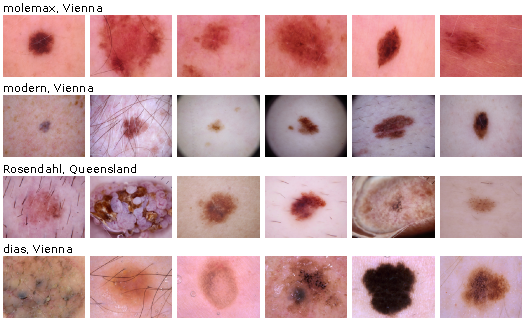
\includegraphics[width=\columnwidth]{figures/fig2_nevi.pdf}
\caption{Benign nevi from the four HAM10000 sources. The diagnosis is the same in every row; colour, skin tone and borders change with the source.}\label{fig:nevi}
\end{figure}

To measure how much accuracy these differences cost in FL, we build a second set of four sites, the mixed sites. Each mixed site keeps nearly the same number of images of each disease as the real site it replaces, but takes its lesions at random from all four sources. The mixed sites therefore have the same sizes, the same diseases and the same images as the real sites; they differ only in that every site now holds images from every source. We call the accuracy that FedAvg on the real sites loses against centralized training of the same model the FL gap. If FedAvg is more accurate on the mixed sites, the gain shows how much of the FL gap comes from differences between image sources.

Fed-ISIC2019 has 23,247 images in eight classes from six centres, four of which are the HAM10000 sources. We build mixed sites there in the same way and use the FLamby metric, which averages the balanced accuracy of the six centres.

\subsection{Backbone and normalization}
We vary the normalization layer of the backbone because our main hypothesis concerns it. A batch-normalization layer, or BN, normalizes its input with a mean and variance that it estimates from the training images and stores in the model. A layer-normalization layer, or LN, normalizes each image using only that image's own features and stores no statistics. In FL, the server averages the stored BN statistics of all sites like any other weight. We hypothesize that when each site's images have their own colour and brightness, its BN statistics adapt to them, and their average fits none of the sites well.

We compare two BN models, EfficientNet-B0 [10] and ResNet-18, and two LN models, ConvNeXt-atto [11] and DeiT-tiny. Because the BN and LN models also differ in architecture, we add a ResNet-50 in two versions with the same architecture and pretraining, one with BN and one with group normalization, which, like LN, normalizes within each image and stores no statistics. Only this pair isolates the effect of normalization. EfficientNet-B0 is our baseline because it is the model used by FLamby. ConvNeXt-atto is our main LN model because it is a convolutional network of similar size, 3.4 million weights against 4.0 million.

All models start from ImageNet weights and are trained on 224-pixel images with AdamW, a learning rate of 0.0003, a batch size of 64 and a cross-entropy loss weighted so that rare classes count more; the ResNet-50 pair uses 160-pixel images to fit a 4 GB GPU. On HAM10000, federated training runs 30 rounds of one local epoch, and we keep the round with the best validation accuracy. On Fed-ISIC2019 we score the model after the last round, as FLamby does. Each setting is run with three random seeds, and five for the baseline and the best model.

\subsection{Privacy}
We first measure how much a model leaks and then add protection. The attacker is the server, or anyone who later obtains the model, and tries to tell whether a given image was used in training. We use the RMIA attack [8], which trains eight extra models on known halves of the training data to learn how a model behaves on images it has not seen. We report the share of training images that the attack finds while wrongly flagging only 1\% of the images that were not used in training.

For protection, each site trains with DP-SGD [2]: at every step, the influence of each image on the update is limited by clipping, and random noise is added. The privacy level is set by $\varepsilon$; a smaller $\varepsilon$ means stronger privacy and more noise. Each site uses its own $\varepsilon$ of 8, 3 or 1 over the whole training. We tried DP on three parts of the network: the last two blocks with the classifier, the last block with the classifier, and the classifier alone. Training only the classifier on top of a frozen backbone means that about nine thousand weights are trained instead of millions, which is expected to make the noise less harmful, and accuracy then depends mainly on how good the frozen features are [7]. With an ImageNet backbone, this gives our private reference. In our proposed version, the same EfficientNet-B0 is first trained on the BCN images of ISIC 2019, public dermoscopy images from a hospital outside our four sites. Before this, we compared these images with all HAM10000 images and found no confirmed duplicate among 7,463 candidate pairs. Only the frozen weights differ between the two private versions.

\section{Results}
Numbers are balanced accuracy on the HAM10000 validation set, averaged over seeds, unless stated otherwise.

\subsection{Source differences explain a large part of the FL gap of BN models}
Moving from the real to the mixed sites recovers 35\% to 49\% of the FL gap for the three BN models and none of it for the two LN models (Table~\ref{tab:dev}). For the BN models, FedAvg is 0.10 to 0.14 below centralized training, and on the mixed sites it gains about 0.05. For the LN models the FL gap is smaller, 0.076 and 0.036, and FedAvg does not improve on the mixed sites.

\begin{table}[t]
\caption{The mixed sites recover part of the FL gap for batch-normalization models only. Real and Mixed: FedAvg on the real and on the mixed sites. Recovered: gain from mixing divided by the FL gap.}\label{tab:dev}
\centering\footnotesize\setlength{\tabcolsep}{3.2pt}
\begin{tabular}{llccccc}
\toprule
Backbone & Norm & Central & Real & Mixed & Gap & Recovered \\
\midrule
EfficientNet-B0 & BN & 0.778 & 0.659 & 0.707 & 0.118 & 40\% \\
ResNet-18 & BN & 0.797 & 0.657 & 0.706 & 0.140 & 35\% \\
ResNet-50 & BN & 0.800 & 0.698 & 0.748 & 0.102 & 49\% \\
ResNet-50 & GN & 0.791 & 0.700 & 0.713 & 0.092 & 15\% \\
ConvNeXt-atto & LN & 0.813 & 0.737 & 0.733 & 0.076 & none \\
DeiT-tiny & LN & 0.779 & 0.742 & 0.698 & 0.036 & none \\
\bottomrule
\end{tabular}
\end{table}

Melanoma, the most dangerous class, is among the classes that lose most. For the EfficientNet-B0 baseline, FL lowers melanoma recall on the test set from 0.645 to 0.380, as the model predicts benign nevus, the largest class, more often. On the mixed sites, melanoma recall rises to 0.499. ConvNeXt-atto keeps more of it, 0.692 against 0.756 with centralized training.

\subsection{Evidence that the loss enters through BN statistics}
Source differences could hurt FedAvg in two ways: the sites could pull the model in different directions during local training, or their BN statistics could differ so much that their average fits no site. The first explanation is not supported. The mixed sites raised the accuracy of EfficientNet-B0 by 0.047, while the cosine similarity between the updates of different sites, which shows whether they point the same way, changed by at most 0.05. Four results support the second explanation. First, the mixed sites help all three BN models and neither LN model. Second, in the ResNet-50 pair, which differs only in normalization, the mixed sites help the BN version by 0.051 in every seed but the group-normalization version by only 0.014, within the variation between seeds. Third, FedBN, which keeps the BN statistics inside each site, gains 0.080 over FedAvg on the real sites but only 0.013 on the mixed sites. Fourth, correcting the colour of each image before training raises FedAvg by 0.024 for EfficientNet-B0 but by only 0.006 for ConvNeXt-atto. These results fit our hypothesis, but they do not prove that the BN statistics are the only cause.

FedBN is not a practical fix, because it needs to know which site a new image comes from. Without this information, using the average prediction of all site models, it scores 0.639 against 0.659 for FedAvg. About 60\% of the FL gap of the BN models remains on the mixed sites, where only the diseases and sizes of the sites differ. FedProx, a common variant of FedAvg, did not reduce it in our tests.

\subsection{The best federated model and the baseline}\label{sec:best}
ConvNeXt-atto, which uses LN, gives the best federated model. With FedAvg it reaches 0.741 with a standard deviation of 0.013 over five seeds, against 0.661 with 0.010 for the EfficientNet-B0 baseline, and 0.662 against 0.597 on the test set (Table~\ref{tab:designs}). With centralized training the two differ by only 0.035, so most of the difference appears in FL. During federated training the baseline stops improving after about ten rounds, while ConvNeXt-atto keeps improving almost until the last round. It is also smaller and faster, about 9 minutes per run against 14 on a 4 GB laptop GPU. Because the two models differ in architecture as well as in normalization, part of this advantage may come from the architecture.

\begin{table}[t]
\caption{Final models on HAM10000. The DP guarantee is at $\varepsilon = 3$.}\label{tab:designs}
\centering\footnotesize\setlength{\tabcolsep}{3.2pt}
\begin{tabular}{lcccc}
\toprule
Model & Weights trained & Val. & Test & DP \\
\midrule
Baseline, EfficientNet-B0 & 4.0 million & 0.661 & 0.597 & no \\
Best federated, ConvNeXt-atto & 3.4 million & 0.741 & 0.662 & no \\
DP classifier, ImageNet features & 8,967 & 0.430 & 0.386 & yes \\
DP classifier, public features & 8,967 & 0.554 & 0.508 & yes \\
\bottomrule
\end{tabular}
\end{table}

On Fed-ISIC2019 the mixed sites again help the BN baseline. In the original FLamby setup, with 9 rounds of 100 local steps, they raise its FedAvg accuracy by 0.030, which is 28\% of its FL gap. With our HAM10000 training settings and three times as many steps, 27 rounds of 100, they recover 42\% of the gap, close to the 40\% on HAM10000, while ConvNeXt-atto gains only 0.008. The advantage of ConvNeXt-atto also needs the longer training. With the FLamby number of steps the two models are close, 0.643 and 0.628, but with three times the steps ConvNeXt-atto leads by 0.043 in the FLamby metric. Counted over all test images together, the two models tie, 0.700 and 0.699, because ConvNeXt-atto is slightly behind at BCN, the largest centre.

\subsection{Adding privacy}
Federated training lowers leakage but does not remove it. While wrongly flagging 1\% of the unused images, RMIA finds 4.3\% of the training images of the federated baseline, against 9.6\% when the same model is trained centrally, and 5.4\% against 7.1\% for ConvNeXt-atto. A formal guarantee therefore still requires DP.

Of the three parts we tried, only DP on the classifier alone kept useful accuracy. With DP on the last one or two blocks, accuracy fell to between 0.15 and 0.24 at every $\varepsilon$ we tried, close to the 0.14 of random guessing. With DP on the classifier and ImageNet features, accuracy falls from 0.617 without DP to 0.430 at $\varepsilon = 3$; clipping alone costs only 0.015 of this, so most of the loss comes from the noise. The best federated model does not help here: with frozen ConvNeXt-atto features, accuracy at $\varepsilon = 3$ is 0.353, below EfficientNet-B0, so both private versions use EfficientNet-B0.

Public dermoscopy features raise private accuracy by 0.12 to 0.13 at each $\varepsilon$ (Figure~\ref{fig:priv}), from 0.430 to 0.554 at $\varepsilon = 3$. Without DP, a classifier on these features reaches 0.710, already above the full FedAvg baseline. This narrows the cost of privacy but does not remove it: at $\varepsilon = 3$ the private model is 0.19 below the best federated model.

\begin{figure}[t]
\centering
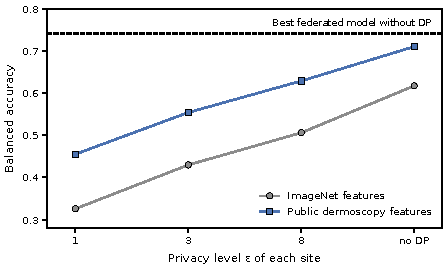
\includegraphics[width=\columnwidth]{figures/fig4_privacy.pdf}
\caption{Balanced accuracy of the DP classifier at each privacy level, with ImageNet features and with public dermoscopy features. The dashed line is the best federated model without DP.}\label{fig:priv}
\end{figure}

\section{Discussion and limitations}
Our results suggest that, for hospitals building a federated skin-lesion model, the choice of backbone can matter more than the choice of FL algorithm. With BN, part of the accuracy lost in FL appears to come from differences between image sources, and it lowers melanoma recall. An LN backbone was much less affected and, unlike FedBN, did not need to know where each image comes from. Benchmarks should also report how long they train, since the FLamby number of steps hid the advantage of the LN model. For privacy, keeping images on site was not enough in our tests. If a formal guarantee is needed, DP at our scale was usable only on the classifier, and the quality of the frozen features largely decided how much accuracy remained. A hospital would still have to choose between the most accurate model and one with a formal guarantee, 0.19 apart in our setting.

These conclusions have limits. Our setting is small, four sites with 8,583 training images, so most differences between single sites are not significant. The mixed sites remove all differences between sources, including patients and photography habits, so we cannot separate the devices from these other factors. The four comparisons support the role of the BN statistics but do not prove it, and apart from the ResNet-50 pair, the BN and LN models also differ in architecture. Mixing sources did not help the LN models: for ConvNeXt-atto it lowered melanoma recall to 0.554 at the same balanced accuracy, and it lowered the accuracy of DeiT-tiny for reasons we could not find. The attack uses extra models trained centrally, so the measured leakage is likely a lower bound, and the public BCN images come from the same ISIC collection as HAM10000.

\section{Conclusion}
We measured where federated learning loses accuracy on real skin-lesion sites and how much a formal privacy guarantee costs. For batch-normalization models, differences between image sources account for 35\% to 49\% of the FL gap, and our results point to the statistics averaged by the server as the main path. A layer-normalization model was much less affected and gave the best federated model, 0.741 against 0.661 for the baseline, and mixing sources helped the baseline again on Fed-ISIC2019. Under DP, public dermoscopy features raised accuracy at $\varepsilon = 3$ from 0.430 to 0.554, still 0.19 below the best model. Code, data splits and run logs are available from the author on request.

{\small
\begin{thebibliography}{99}
\setlength{\itemsep}{1pt}
\bibitem{r1} H. B. McMahan, E. Moore, D. Ramage, S. Hampson, and B. Agüera y Arcas, ``Communication-efficient learning of deep networks from decentralized data,'' in \textit{Proc. 20th Int. Conf. Artificial Intelligence and Statistics (AISTATS)}, PMLR vol. 54, 2017, pp. 1273--1282. Available: \url{https://proceedings.mlr.press/v54/mcmahan17a.html}
\bibitem{r2} M. Abadi et al., ``Deep learning with differential privacy,'' in \textit{Proc. ACM SIGSAC Conf. Computer and Communications Security (CCS)}, 2016, pp. 308--318, doi: \href{https://doi.org/10.1145/2976749.2978318}{10.1145/2976749.2978318}.
\bibitem{r3} J. Ogier du Terrail et al., ``FLamby: Datasets and benchmarks for cross-silo federated learning in realistic healthcare settings,'' in \textit{Advances in Neural Information Processing Systems (NeurIPS)}, Datasets and Benchmarks Track, vol. 35, 2022, pp. 5315--5334. Available: \url{https://proceedings.neurips.cc/paper_files/paper/2022/hash/232eee8ef411a0a316efa298d7be3c2b-Abstract.html}
\bibitem{r4} P. Tschandl, C. Rosendahl, and H. Kittler, ``The HAM10000 dataset, a large collection of multi-source dermatoscopic images of common pigmented skin lesions,'' \textit{Sci. Data}, vol. 5, art. no. 180161, 2018, doi: \href{https://doi.org/10.1038/sdata.2018.161}{10.1038/sdata.2018.161}.
\bibitem{r5} K. Hsieh, A. Phanishayee, O. Mutlu, and P. Gibbons, ``The non-IID data quagmire of decentralized machine learning,'' in \textit{Proc. 37th Int. Conf. Machine Learning (ICML)}, PMLR vol. 119, 2020, pp. 4387--4398. Available: \url{https://proceedings.mlr.press/v119/hsieh20a.html}
\bibitem{r6} X. Li, M. Jiang, X. Zhang, M. Kamp, and Q. Dou, ``FedBN: Federated learning on non-IID features via local batch normalization,'' in \textit{Proc. Int. Conf. Learning Representations (ICLR)}, 2021. Available: \url{https://openreview.net/pdf/37e144ecec7a76ce5093d4ec328649e8ef208a5b.pdf}
\bibitem{r7} F. Tramèr and D. Boneh, ``Differentially private learning needs better features (or much more data),'' in \textit{Proc. Int. Conf. Learning Representations (ICLR)}, 2021. Available: \url{https://openreview.net/forum?id=YTWGvpFOQD-}
\bibitem{r8} S. Zarifzadeh, P. Liu, and R. Shokri, ``Low-cost high-power membership inference attacks,'' in \textit{Proc. 41st Int. Conf. Machine Learning (ICML)}, PMLR vol. 235, 2024, pp. 58244--58282. Available: \url{https://proceedings.mlr.press/v235/zarifzadeh24a.html}
\bibitem{r9} Z. Chen, C. Yang, M. Zhu, Z. Peng, and Y. Yuan, ``Personalized retrogress-resilient federated learning toward imbalanced medical data,'' \textit{IEEE Trans. Med. Imag.}, vol. 41, no. 12, pp. 3663--3674, 2022, doi: \href{https://doi.org/10.1109/TMI.2022.3192483}{10.1109/TMI.2022.3192483}.
\bibitem{r10} M. Tan and Q. Le, ``EfficientNet: Rethinking model scaling for convolutional neural networks,'' in \textit{Proc. 36th Int. Conf. Machine Learning (ICML)}, PMLR vol. 97, 2019, pp. 6105--6114. Available: \url{https://proceedings.mlr.press/v97/tan19a.html}
\bibitem{r11} Z. Liu, H. Mao, C.-Y. Wu, C. Feichtenhofer, T. Darrell, and S. Xie, ``A ConvNet for the 2020s,'' in \textit{Proc. IEEE/CVF Conf. Computer Vision and Pattern Recognition (CVPR)}, 2022, pp. 11976--11986. Available: \url{https://openaccess.thecvf.com/content/CVPR2022/html/Liu_A_ConvNet_for_the_2020s_CVPR_2022_paper.html}
\end{thebibliography}}
\end{document}
